\documentclass[a4paper,12pt]{article}
\usepackage[utf8]{inputenc}
\usepackage[T1]{fontenc}
\usepackage[polish]{babel}
\usepackage{geometry}
\usepackage{graphicx}
\usepackage{float}
\usepackage{amsmath}
\usepackage{amssymb}
\usepackage{hyperref}
\usepackage{booktabs}
\usepackage{caption}
\usepackage{subcaption}
\usepackage{listings}
\usepackage{xcolor}

\geometry{margin=2.5cm}

\title{\textbf{Sprawozdanie: Laboratorium 4}\\Algorytmy optymalizacji dyskretnej\\Maksymalny przepływ i skojarzenia}
\author{Paweł Grzegory}
\date{\today}

\begin{document}

\maketitle

\tableofcontents
\newpage

\section{Wstęp}
Celem laboratorium było zbadanie problemów maksymalnego przepływu w sieciach oraz maksymalnego skojarzenia w grafach dwudzielnych. Zaimplementowano algorytmy kombinatoryczne (Edmonds-Karp, Hopcroft-Karp, Shortest Augmenting Path) oraz porównano ich wydajność z podejściem opartym na programowaniu liniowym (LP) przy użyciu solvera GLPK. Badania przeprowadzono na grafach hiperkostki (dla przepływu) oraz losowych grafach dwudzielnych.

\section{Zadanie 1: Algorytm Edmondsa-Karpa}

\subsection{Opis implementacji i złożoność}
Zaimplementowano algorytm Edmondsa-Karpa, będący specjalizacją metody Forda-Fulkersona. Kluczową cechą tej implementacji jest sposób wyboru ścieżki powiększającej w sieci residualnej $G_f$.

Algorytm działa w pętli:
\begin{enumerate}
    \item Konstruuje sieć residualną na podstawie aktualnego przepływu.
    \item Uruchamia przeszukiwanie wszerz (BFS) startując z wierzchołka źródłowego $s$, aby znaleźć ścieżkę do ujścia $t$ o \textbf{minimalnej liczbie krawędzi}.
    \item Jeśli ścieżka istnieje, identyfikuje tzw. \textit{wąskie gardło} (krawędź o minimalnej przepustowości residualnej $c_f(u,v)$ na ścieżce) i zwiększa przepływ wzdłuż tej ścieżki.
    \item Procedura powtarza się, aż w sieci residualnej nie będzie ścieżki z $s$ do $t$.
\end{enumerate}

\textbf{Złożoność obliczeniowa:} $O(V E^2)$.
Dla badanej hiperkostki $H_k$:
\begin{itemize}
    \item Liczba wierzchołków $V = 2^k$.
    \item Liczba krawędzi $E = k \cdot 2^{k-1}$.
\end{itemize}
Wraz ze wzrostem $k$, liczba wierzchołków rośnie wykładniczo ($2^{16} = 65\,536$), co powoduje gwałtowny wzrost czasu obliczeń.

\subsection{Wyniki eksperymentów}
Badania przeprowadzono dla $k \in \{1, \dots, 16\}$.

\begin{figure}[H]
    \centering
    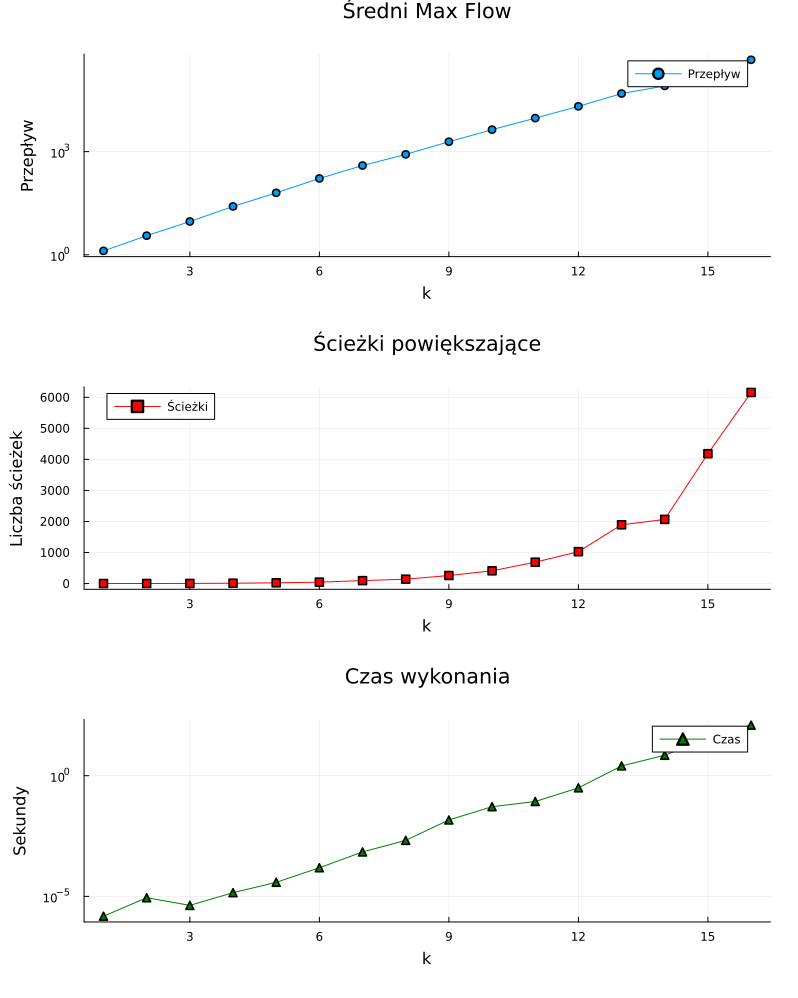
\includegraphics[width=0.9\textwidth]{results_k1_k16.png}
    \caption{Zależność maksymalnego przepływu, liczby ścieżek i czasu wykonania od wymiaru hiperkostki $k$.}
    \label{fig:ek_results}
\end{figure}

\textbf{Wnioski:}
Czas wykonania rośnie wykładniczo, co widać na wykresie w skali logarytmicznej (liniowy wzrost na wykresie logarytmicznym oznacza zależność wykładniczą). Liczba ścieżek powiększających również rośnie, ale wolniej niż czas przeszukiwania grafu.

\newpage
\section{Zadanie 2: Algorytm Hopcrofta-Karpa}

\subsection{Opis implementacji}
Do znalezienia maksymalnego skojarzenia w grafie dwudzielnym $G=(V_1 \cup V_2, E)$ wykorzystano algorytm Hopcrofta-Karpa. Jest to jeden z najefektywniejszych algorytmów dla tego problemu.

Algorytm przebiega w fazach, z których każda składa się z dwóch etapów:
\begin{enumerate}
    \item \textbf{BFS (Podział na warstwy):} Przeszukiwanie wszerz startuje ze wszystkich wolnych (nieskojarzonych) wierzchołków w $V_1$. Celem jest znalezienie długości najkrótszej ścieżki powiększającej oraz zbudowanie grafu warstwowego.
    \item \textbf{DFS (Szukanie ścieżek):} Przeszukiwanie w głąb wykorzystuje graf warstwowy do znalezienia \textbf{maksymalnego zbioru rozłącznych wierzchołkowo} ścieżek powiększających o minimalnej długości wyznaczonej przez BFS.
\end{enumerate}

\textbf{Złożoność obliczeniowa:} $O(E\sqrt{V})$. Jest to znacząca poprawa względem prostego zastosowania algorytmu Forda-Fulkersona ($O(VE)$).

\subsection{Wyniki eksperymentów}
Przeprowadzono testy dla $k \in \{3, \dots, 10\}$ oraz różnych stopni wierzchołków $i$.

\begin{figure}[H]
    \centering
    \begin{subfigure}[b]{0.48\textwidth}
        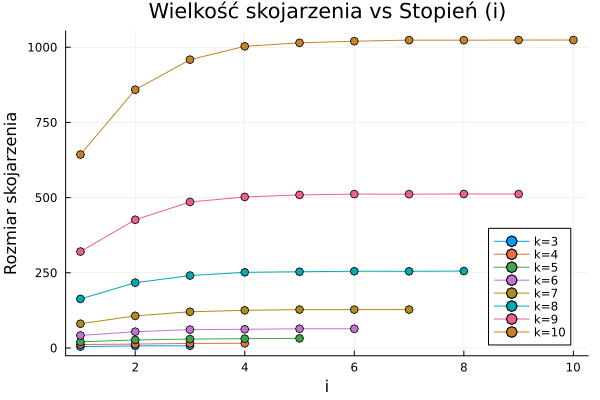
\includegraphics[width=\textwidth]{matching_size_vs_i.png}
        \caption{Wielkość skojarzenia w zależności od stopnia $i$.}
    \end{subfigure}
    \hfill
    \begin{subfigure}[b]{0.48\textwidth}
        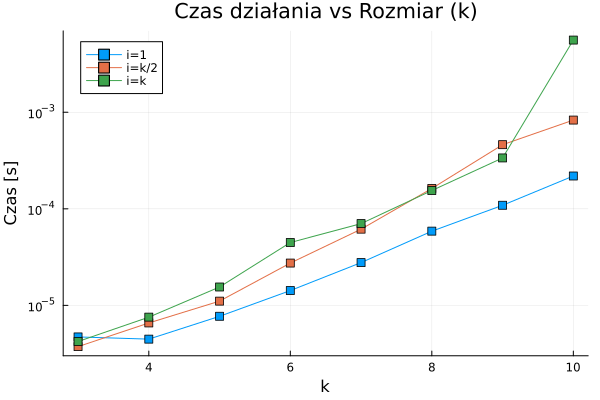
\includegraphics[width=\textwidth]{execution_time_vs_k.png}
        \caption{Czas działania w zależności od rozmiaru $k$.}
    \end{subfigure}
    \caption{Wyniki dla algorytmu Hopcrofta-Karpa.}
    \label{fig:hk_results}
\end{figure}

\textbf{Wnioski:}
Algorytm działa bardzo szybko nawet dla dużych grafów dwudzielnych ($k=10$). Wykres wielkości skojarzenia pokazuje nasycenie – powyżej pewnego stopnia $i$, skojarzenie obejmuje prawie wszystkie wierzchołki ("perfect matching").

\newpage
\section{Zadanie 3: Modele Programowania Liniowego (LP)}

Wygenerowano modele LP w formacie zgodnym z solverem GLPK (za pomocą biblioteki JuMP). Poniżej przedstawiono opis matematyczny oraz uzasadnienie przyjętych warunków.

\subsection{Model Maksymalnego Przepływu}
Niech $G=(V, A)$ będzie siecią z przepustowościami $c_{uv}$.
\textbf{Zmienne decyzyjne:} $f_{uv} \in \mathbb{R}$ – przepływ na łuku $(u,v)$.

\textbf{Sformułowanie problemu:}
\begin{equation}
\begin{aligned}
\text{Maksymalizuj:} \quad & \sum_{(s,v) \in A} f_{sv} \\
\text{Pod warunkiem:} \quad & \sum_{(v,u) \in A} f_{vu} = \sum_{(u,w) \in A} f_{uw} \quad \forall u \in V \setminus \{s, t\} \\
& 0 \le f_{uv} \le c_{uv} \quad \forall (u,v) \in A
\end{aligned}
\end{equation}

\textbf{Wyjaśnienie warunków:}
\begin{itemize}
    \item \textbf{Funkcja celu:} Chcemy zmaksymalizować całkowity wypływ ze źródła $s$, co jest równoznaczne z wartością przepływu w sieci.
    \item \textbf{Bilans przepływu (Kirchhoffa):} Dla każdego węzła pośredniego (niebędącego źródłem ani ujściem), suma wpływających jednostek musi być równa sumie wypływających. Przepływ nie może "znikać" ani "powstawać" w węzłach pośrednich.
    \item \textbf{Ograniczenie przepustowości:} Przepływ $f_{uv}$ nie może przekroczyć fizycznej pojemności krawędzi $c_{uv}$ oraz musi być nieujemny (przepływ jednokierunkowy).
\end{itemize}

\subsection{Model Maksymalnego Skojarzenia}
Dla grafu dwudzielnego $G=(V_1 \cup V_2, E)$.
\textbf{Zmienne decyzyjne:} $x_{uv} \in \{0, 1\}$ – zmienna binarna.

\textbf{Sformułowanie problemu:}
\begin{equation}
\begin{aligned}
\text{Maksymalizuj:} \quad & \sum_{(u,v) \in E} x_{uv} \\
\text{Pod warunkiem:} \quad & \sum_{v \in N(u)} x_{uv} \le 1 \quad \forall u \in V_1 \\
& \sum_{u \in N(v)} x_{uv} \le 1 \quad \forall v \in V_2 \\
& x_{uv} \in \{0, 1\}
\end{aligned}
\end{equation}

\textbf{Wyjaśnienie warunków:}
\begin{itemize}
    \item \textbf{Zmienne binarne:} $x_{uv}=1$ oznacza, że krawędź $(u,v)$ została wybrana do skojarzenia, $0$ w przeciwnym wypadku.
    \item \textbf{Ograniczenia ($\le 1$):} Z definicji skojarzenia, każdy wierzchołek może być końcem co najwyżej jednej krawędzi należącej do skojarzenia. Sumujemy więc zmienne $x$ incydentne do danego wierzchołka i wymuszamy, by suma ta wynosiła 0 lub 1.
\end{itemize}

\subsection{Porównanie wydajności: Algorytmy vs GLPK}
\begin{figure}[H]
    \centering
    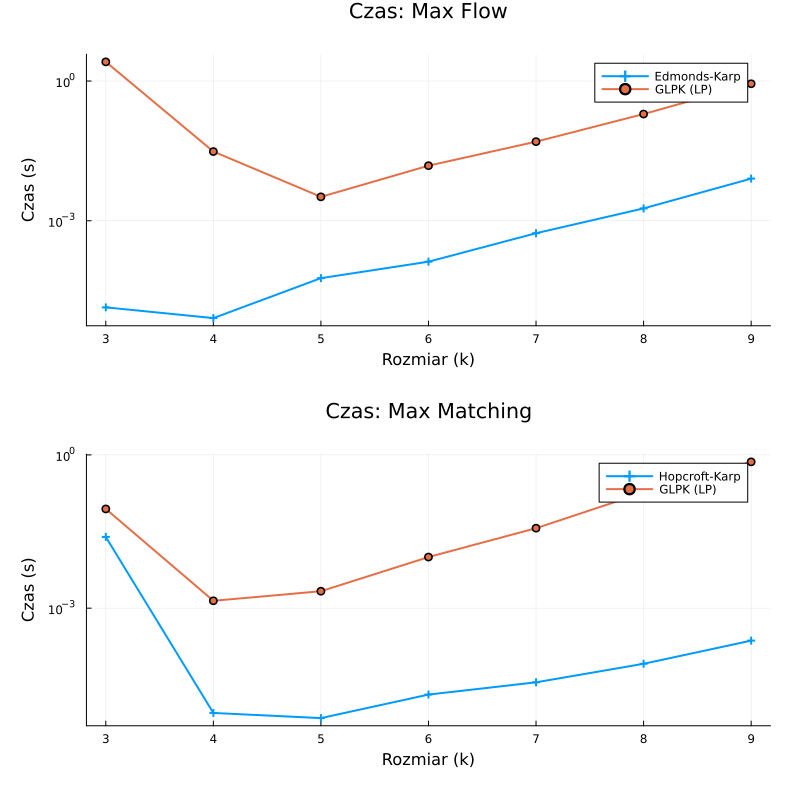
\includegraphics[width=0.8\textwidth]{comparison_lp_vs_algo.png}
    \caption{Porównanie czasu działania algorytmów kombinatorycznych i LP.}
    \label{fig:lp_vs_algo}
\end{figure}

\textbf{Wnioski:} Algorytmy dedykowane (EK, HK) są rzędy wielkości szybsze od solvera GLPK (metoda simpleks). Solvery LP są ogólnego przeznaczenia i nie wykorzystują specyficznej struktury grafu tak efektywnie. Wyniki liczbowe były identyczne.

\newpage
\section{Zadanie 4: Algorytm Shortest Augmenting Path (SAP)}

\subsection{Opis algorytmu i zastosowane optymalizacje}
W ramach zadania dodatkowego zaimplementowano algorytm \textit{Shortest Augmenting Path} (SAP). Jest to algorytm, który podobnie jak Edmonds-Karp szuka najkrótszych ścieżek, ale robi to efektywniej dzięki wykorzystaniu funkcji odległości (distance labels).

Algorytm utrzymuje dla każdego wierzchołka $u$ etykietę $d(u)$, będącą dolnym oszacowaniem odległości od $u$ do ujścia $t$. Zastosowano następujące optymalizacje zapewniające złożoność $O(V^2 E)$:

\begin{enumerate}
    \item \textbf{Exact Distance Labels (BFS wsteczny):} Etykiety są inicjalizowane BFS-em wstecznym z ujścia, co daje dokładne odległości na starcie.
    \item \textbf{Current Arc Optimization:} Każdy wierzchołek pamięta wskaźnik do ostatnio sprawdzonej krawędzi, unikając wielokrotnego przeglądania tych samych łuków.
    \item \textbf{Gap Heuristic:} Jeśli licznik wierzchołków o danej odległości $k$ spadnie do zera, wszystkie wierzchołki o odległości $>k$ stają się nieosiągalne (tzw. luka), co pozwala przerwać obliczenia lub relubować wierzchołki.
\end{enumerate}

\subsection{Porównanie: Edmonds-Karp vs SAP}

\begin{figure}[H]
    \centering
    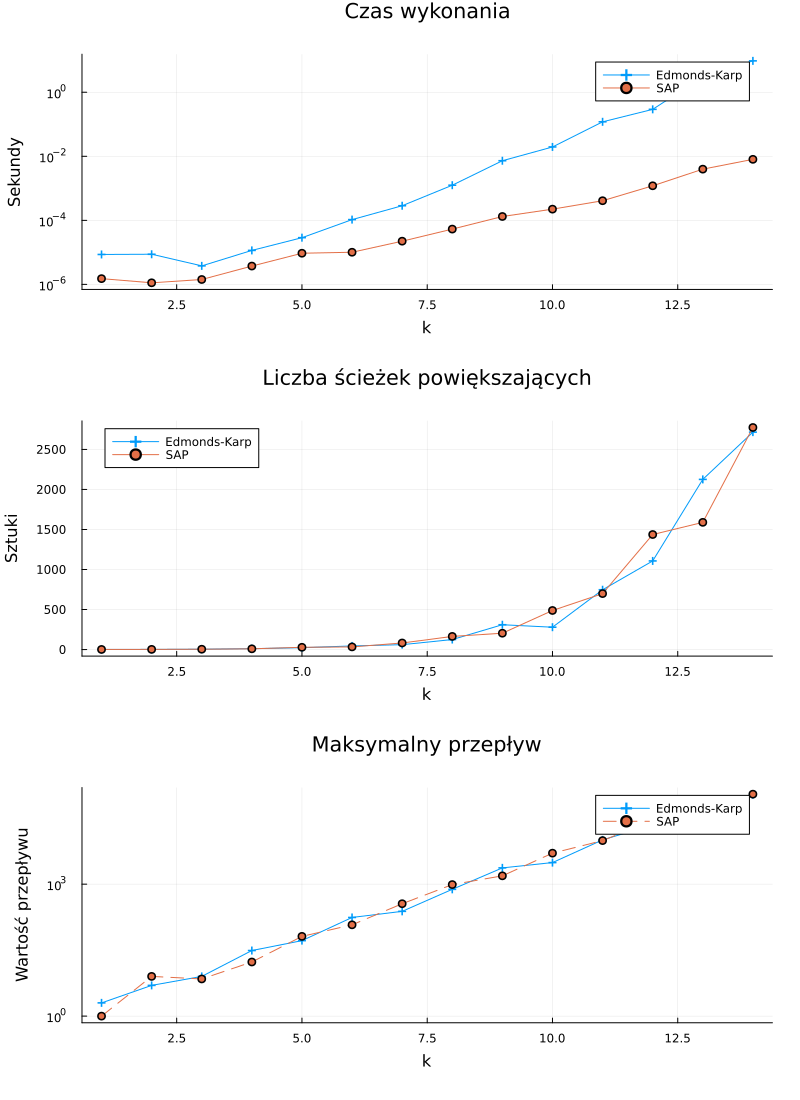
\includegraphics[width=0.9\textwidth]{full_comparison_ek_vs_sap.png}
    \caption{Bezpośrednie porównanie wydajności algorytmów EK i SAP.}
    \label{fig:sap_vs_ek}
\end{figure}

\textbf{Wnioski:}
Algorytm SAP (linia pomarańczowa) osiąga znacznie lepsze czasy dla dużych wartości $k$. Mechanizm "Gap Heuristic" oraz brak konieczności uruchamiania pełnego BFS w każdej iteracji (jak w EK) sprawiają, że SAP jest znacznie bardziej skalowalny dla gęstych grafów typu hiperkostka.

\section{Podsumowanie}
W laboratorium zbadano trzy klasy algorytmów. Dedykowane algorytmy kombinatoryczne (Hopcroft-Karp, SAP) okazały się bezkonkurencyjne czasowo. Podejście LP, choć najprostsze w modelowaniu (deklaratywne), jest nieefektywne dla dużych instancji problemów grafowych. Implementacja SAP z heurystykami pozwoliła na rozwiązanie problemu dla $k=14$ w czasie rzędu milisekund, podczas gdy Edmonds-Karp zaczynał zwalniać.

\end{document}